\chapter{Literature Review II}
\label{chap:literature}



%\section{Automated Random Testing Tools}
\section{Tools for Automated Random Testing}
A number of open-source and commercial random testing tools that automatically generate test cases, reported in the literature, are briefly described in the following section.


\subsection{JCrasher}
JCrasher is an automatic robustness testing tool developed by Csallner and Smaragadakis \cite{Pacheco2007b}. JCrasher tries to crash the Java program with random input and exceptions thrown during the process are recorded. The exceptions are then compared with the list of acceptable standards, defined in advance as heuristics. The undefined runtime exceptions are considered as errors. Since users interact with programs through its public methods with different kind of inputs, therefore, JCrasher is designed to test only the public methods of the SUT with random inputs.

\begin{figure}[h]
	\centering
	\includegraphics[width=15cm, height=7cm]{chapter3/JCrasher.png}
	\caption{Illustration of robustness testing of Java program with JCrasher~\cite{Pacheco2007b}}
	\label{fig:JCrasher}
\end{figure}

Figure~\ref{fig:JCrasher} illustrates the working of JCrasher by testing a {\it T.java} program. The source file is first compiled using {\it javac} and the byte code obtained is passed as input to JCrasher. The JCrasher, with the help of Java reflection~\cite{chan1999java}, analyse all the methods declared by class {\it T} using methods transitive parameter types { \it P} to generate the most appropriate test data set which is written to a file {\it TTest.java}. The file is compiled and executed by JUnit. All the exceptions produced during test case executions are collected and compared with robustness heuristic for any violation which is reported as error.\\

\noindent JCrasher is a pioneering tool with the capability to perform fully automatic testing, including test case generation, execution, filtration to report generation. JCrasher has the novelty to generate test cases as JUnit files which can also be easily read and used for regression testing. Another important feature of JCrasher is to execute each new test on a ``clean slate" ensuring that the changes made by the previous tests do not affect the new test.  

% check parameter space or parameter graph in the figure???


\subsection{Jartege}
Jartege (\uline{Ja}wa~\uline{r}andom~\uline{te}st~\uline{ge}nerator)~\cite{Oriat2004} is an automated testing tool that randomly generates unit tests for Java classes with contracts specified in Java Modelling Language (JML). The contracts include methods pre- and post-conditions and class invariants. Initially Jartege uses the contracts to eliminate irrelevant test cases and later on the same contracts serve as test oracle to differentiate between errors and false positives. Jartege uses simple random testing to test classes and generate test cases. In addition, it parametrise its random aspect in order to prioritise testing specific part of the class or to get interesting sequences of calls. The parameters include the following: 
\begin{itemize}
\item Operational profile of the classes i.e. the likely use of the class under test by other classes.  
\item Weight of the class and the method under test. Higher weight prioritizes the class or method over lower weight during test process. 
\item Probability of creating new objects during test process. Low probability means creation of fewer objects and more re-usability for different operations while high probability means numerous new objects with less re-usability.
\end{itemize}

\noindent The Jartege technique evaluates a class by entry pre-condition and internal pre-conditions. Entry pre-conditions are the contracts to be met by the generated test data for testing the method while internal pre-conditions are the contracts which are inside the methods and their violation are considered as error either in the method or in the specification. The Jartege checks for errors in program code as well as in specifications and the Junit tests produced by Jartege can be used later as regression tests. Its limitation is the requirement of prior existence of the program JML specifications.

\subsection{Eclat}
Eclat~\cite{Pacheco2005} is an automated testing tool which generates and classifies unit tests for Java classes. The process is accomplished in three main components. In the first component, it selects a small subset of test inputs, likely to reveal faults in the given SUT, from a large set.

\begin{figure}[h]
	\centering
	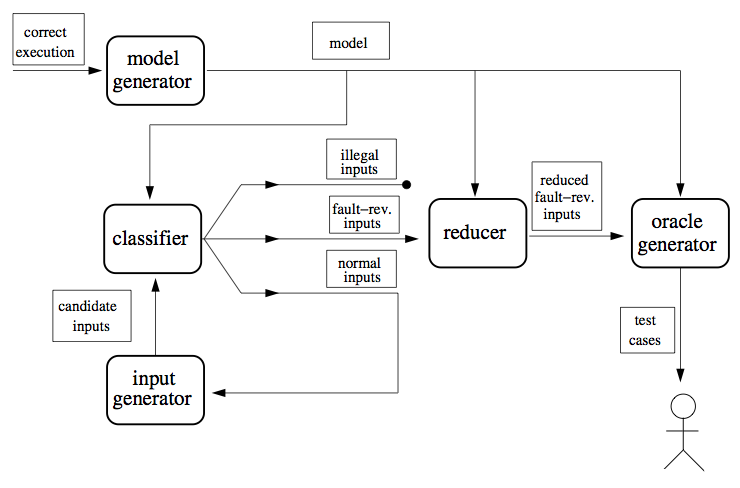
\includegraphics[width=15cm, height=9cm]{chapter3/eclat_working.png}
	\caption{Main component of Eclat contributing to generate test input~\cite{Pacheco2005}}
	\label{fig:eclat}
\end{figure}


\noindent The tool takes a software and a set of test cases for which the software runs properly. It then creates an operational model based on the correct software operations and apply the test data. If the operational pattern of execution of the test data differs from the model, the following three outcomes may be possible: (a) it sight a fault in the given SUT, (b) it might produce normal operations despite model violation, (c) it might be an illegal input that the program cannot handle. (note for author extend 2nd and 3rd component)
In the second component of the process, reducer function is used to discard any redundant input, leaving only a single input per operational pattern. In third component the acquired test inputs are converted into test cases, by creation of oracle, to determine the success or failure of the test. \\
\indent Eclat was compared with JCrasher by executing nine programs on  both tools individually~\cite{Pacheco2007b}. Based on the experimental results it was revealed that Eclat perform better than JCrasher. On the average, Eclat selected 5.0 inputs per run out of which 30\% revealed faults, while JCrasher selected 1.13 inputs per run out of which 0.92\% of those revealed faults. The limitation of Eclat is dependence on the initial pool of correct test cases and existence of any errors in the pool may lead to the creation of wrong operational model which will adversely affect the testing process.   

%\subsection{JTest}
%Parasoft Jtest is a commercial tool that automatically generates and execute unit tests. It can be easily integrated to Java IDEs like Eclipse where it provide two main functionalities, i.e. Static Analysis, Unit testing and code coverage. [25]
%In static analysis Jtest takes a complete project or set of classes as input and compares it with a list of built-in rules. The statement violating any of these rules is an error. It also suggests probable fixes for the detected fault.
%For unit testing it takes a class as an input and processes a number of scenarios against it to generate and execute unit tests. Once unit tests are executed they become the part of regression test for future reference.
%Jtest also shows the code coverage of the program by colour coding the statements that are not executed by the unit tests.


\subsection{Randoop Tool}
Random tester for Object Oriented Programs (RANDOOP) is the tool used for implementing FDRT technique~\cite{Pacheco2007b}. RANDOOP is a fully automatic tool, capable of testing Java classes and .Net binaries. It takes as input a set of classes, contracts, filters and time limit while its output is a suite of JUnit and NUnit for Java and .Net program respectively. Each unit test in a test suite is a sequence of method calls (hereafter referred as sequence). RANDOOP build the sequence incrementally by randomly selecting a public method from the class under test and arguments for these methods are selected from the predefined pool in case of primitive types and a sequence or null value in case of reference type. RANDOOP maintains two sets called ErrorSeqs and NonErrorSeqs to record the feedback. It extends ErrorSeqs set in case of contract or filter violation and NonErrorSeqs set when no violation is recorded in the feedback. The use of this dynamic feedback evaluation at runtime brings an object to very complex and interesting state. On test completion it produce ErrorSeqs and NonErrorSeqs as JUnit/NUnit test suite. In terms of coverage and number of faults discovered, RANDOOP implementing FDRT was compared with random testing of JCrasher and JavaPathFinder~\cite{visser2004test}. In their experiments, 14 libraries of both Java and .Net were evaluated. The results showed that RANDOOP achieved more coverage than JCrasher in behavioural, branch coverage and faults detection. It can achieve on par coverage with systematic approaches like JavaPathFinder. RANDOOP also has an edge over model checking for its ability to easily search large input domains.

\subsection{QuickCheck Tool}
QuickCheck~\cite{Claessen2000} is a lightweight random testing tool used for testing of Haskell programs~\cite{Hudak2007}. Haskell is a functional programming language where programs are evaluated by using expressions rather than statements as in imperative programming. In Haskell most of the functions are pure except the IO functions, thus main focus of the tool is on testing pure functions. These are the functions which depend on its input parameters and make changes to them only. QuickCheck tool is designed to have a simple domain-specific language of testable specifications embedded in Haskell. This language is used to define expected properties of the functions under test - for example, reversing a list with single element must result in the same list.\\ %(author check the definition of pure functions)\\
\indent The QuickCheck takes function to be tested and properties of the program defined by tester (Haskell functions) as input. The tool uses built-in random generator to generate effective test data, however, to get adequate coverage in the case of custom data types, the testers can also develop their own generator. On executing the function with test data, the tester defined properties must hold for the function to be correct. Any violation of the defined properties suggest error in the function.



% The function is executed against the generated test data. The QuickCheck evaluates and declares a fault in the function where a test case violates the set properties.   



%\subsection{AgitarOne}
%AgitarOne is a commercial tool that automatically generates unit tests. It has a Junit Generator engine that can create 25,000 lines or more of Junit per hour [29]. It can be easily integrated into famous IDE like Eclipse. It takes as input, classes under test, time and optionally any knowledge or test cases that has a positive influence on the performance of the testing process. The generated Junit tests can be run from the same IDE and can also be used for later regression testing. The GUI interface is called a dashboard which provides in depth knowledge of the tests conducted, failures detected, alerts and the archieves of the tests conducted earlier. It also shows the coverage obtained after executing the Junits against the code under test.

\subsection{Autotost Tool}
The Autotest tool, based on Formal Automated testing is used to test Eiffel language programs~\cite{Ciupa2007}. The Eiffel language uses the concept of contracts which is effectively utilized by Autotest - for example the auto generated input is filtered using pre-conditions and unwanted test input is discarded. The contracts are also used as test oracle to determine if the test is pass or fail. Beside automated testing the Autotest also allow the tester to manually write the test cases to target specific behaviour or section of the code. The Autotest scope can be a single method/class or cluster of methods/classes as inputs, it then automatically generate test input data according to the requirement of the methods or classes.

\begin{figure}[h]
	\centering
	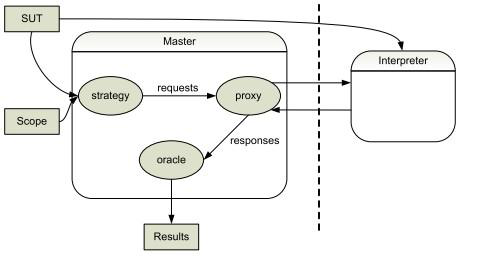
\includegraphics[width=13cm, height=7cm]{chapter3/autotest.png}
	\caption{Architecture of Autotest}
	\label{fig:autotest}
\end{figure}

\noindent According to Figure~\ref{fig:autotest}~\cite{Leitner2007}, the architecture of Autotest tool can be split into the following main parts:
\begin{enumerate}
\item \textbf{Testing Strategy:} is a pluggable component where testers can fit any strategy according to their testing requirements. The strategy contains the directions for testing - for example what instructions should be executed on the SUT. Using the information the strategy synthesize test cases and forward it to the proxy. The default strategy creates test cases that uses random input to exercise the classes under test.
\item \textbf{Proxy:} handles inter-process communication. It receives execution requests from the strategy and forward them to the interpreter. The execution results are sent to the oracle.
\item \textbf{Interpreter:} execute instructions on the SUT. The most common instructions include: create object, invoke routine and assign result. The interpreter process is kept separate to increase robustness.
\item \textbf{Oracle:} is based on contract-based testing. It evaluate the results to see if they satisfy the contracts or not. The outcome of the tests are formatted in HTML and stored on disk.
\end{enumerate}

\subsection{TestEra Tool}
TestEra~\cite{Khurshid2004} is a novel framework for auto generation and evaluation of test inputs for a Java program. It takes methods specifications, integer value and the method under test as input. It uses pre-conditions of a method to generate all non isomorphic valid test input to the specified limit. The test inputs are executed on the method and the results are compared against the postconditions of the method serving as oracle. Any test case that fails to satisfy postcondition is considered as a fault. 

TestEra uses the Alloy modelling language~\cite{jackson2001micromodularity} to express constraints on test inputs and Alloy Analyser tool~\cite{jackson2000alcoa} to solve these constraints and generate test inputs. Alloy Analyzer performs the following three functions: (a) it translates Alloy predicates into propositional formulas, i.e. constraints where all variables are boolean; (b) it evaluates the propositional formulas to find its outcome; (c) it translates each outcome from propositional domain into the relational domain.

\begin{figure}[h]
	\centering
	\includegraphics[width=13cm, height=7.5cm]{chapter3/testera.png}
	\caption{Architecture of TestEra}
	\label{fig:testera}
\end{figure}


TestEra and Korat are similar tools because they both uses program specifications to guide the auto generation of test inputs. However they are different from Jartege and AutoTest which uses specifications to filter and truncate the unnecessary random generated inputs. While the tools use program specifications differently for test input generation, they all uses it in a similar way for oracle. 


%Testera use specifications to guide the automatic generation of test inputs. It uses Alloy language for specification and Alloy Analyser to generate all non-isomorphic instances for a given size according to the specification automatically. Then, TestEra translate the instances to Java input as test cases for the program under test. After executing the test, TestEra then translate the outputs back to Alloy and Alloy Analyzer check the input and output against the correctness criteria given in Alloy. When it detects a violation, TestEra generates report in the form of concrete counterexamples. Figure 2.6 [50] illustrates the basic framework of TestEra.

\subsection{Korat Tool} % please read thesis of khurshid in Mendeley in phd thesis section for more information.
Korat~\cite{Boyapati2002} is a novel framework for automated testing of Java programs based on their formal specifications~\cite{chang1999structural}. Korat and TestEra~\cite{Khurshid2004} were developed by the same team and both performs specification based testing. The difference however is that Korat uses Java Modelling Language (JML) while TestEra uses Alloy Modelling Language for specifications. Korat uses bounded-exhaustive testing \cite{khurshid2001checking} in which the code is tested against all possible inputs within the given small bound.

Korat generate structurally complex inputs by solving imperative predicates. An imperative predicate is a piece of code that takes a structure as input and evaluates to a boolean value. Korat takes imparative predicate and additionally a finitization value, that bounds the size of the structures that are inputs to the predicate, as input. It systematically explore the predicates input space and generate all non isomorphic inputs (inherently distinct inputs in the same input domain) for which the predicates return true. The core part of Korat monitors execution of the predicates on candidate inputs to filter the inputs based on the fields accessed during executions. These inputs are taken as test cases. Korat depends or developers written {\it repOK()} and {\it checkRep()} methods, where {\it repOK()} is used to check the class invariants and {\it checkRep()} is used to verify the post-conditions to validate the correctness of the test case. 

The key benefit of Korat and TestEra, representation level approaches, is that no existing set of operations are required to create input values and therefore they can achieve to create input values that may be difficult or impossible using a given set of operations. However, The only disadvantage to this approach is the requirement of significant amount of manual efforts \cite{pacheco2009directed}.    

%As the test start, it uses methods pre-condition to generate all non-isomorphic test cases up to a given size. It then executes each of the test case and compare the obtained results to the methods post-condition, which serves as an oracle to evaluate the correctness of each test case. 

%%%%%%%%%%%%%%%%%%%%%%%%%%%%%%%%%%%%%%%%%%%%%%
%																						 %
%																						 %			
% YETI Section Starts here									 %
%																						 %		
%																						 %
%%%%%%%%%%%%%%%%%%%%%%%%%%%%%%%%%%%%%%%%%%%%%%


\section{YETI Overview}
YETI stands for York Extensible Testing Infrastructure. It is an automated random testing tool developed in Java that is capable of testing programs written in Java, JML and .NET languages~\cite{Oriol2010c}. YETI takes program byte code as input and execute it with random generated but type-correct inputs to find a fault. It runs at a high level of performance with $10^6$ calls per minute on Java code. One of its prominent feature is Graphical User Interface (GUI) for user friendliness along with the option to change testing process in real time. It can also distribute large testing tasks in cloud for parallel execution~\cite{Oriol2010}. The following sections briefly describe internal working and execution of YETI tool. 

\begin{figure}[h]
	\centering
	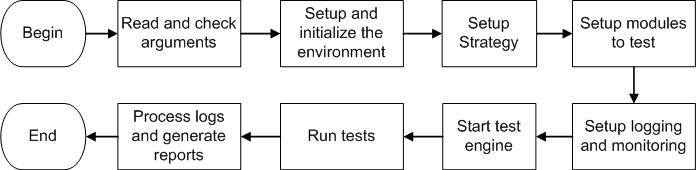
\includegraphics[width=14.5cm, height=3.5cm]{chapter3/yetiOverview.png}
	\caption{YETI test cycle}
	\label{fig:yetiOverview}
\end{figure}


\subsection{Main Components of YETI Tool}
YETI has been designed with an emphasis on extensibility to facilitate future growth. It is therefore divided into three main components: the core infrastructure, strategies and language-specific bindings which are loosely coupled to easily accommodate new languages, strategies and environments. The environment defines the procedure of extracting information from the meta-data of the classes under test and providing it to the core infrastructure. 

\begin{figure}[h]
	\centering
	\includegraphics[width=13cm, height=7.5cm]{yetiMainModules.png}
	\caption{YETI main modules}
	\label{fig:yetiMainModules}
\end{figure}

\subsubsection{YETI Core Infrastructure}
The core infrastructure is responsible for managing the test process and generation of reports. It depends on the following classes to achieve its task.
{\textbf{Yeti:}} It is the fist class in contact after the test command is issued by the user. It contains the main method of YETI which on execution parses the supplied command with options and execute the specific bindings to test the particular language requested in the command.
{\textbf{YetiLog:}} It is the class that facilitate printing debug and testing logs of the current test session. 
{\textbf{YetiLogProcessor:}} It is an interface for processing test logs.
{\textbf{YetiEngine:}} It is the class which make calls for a given number of time or specified amount of time in the command.
{\textbf{YetiTestManager:}} It is the class that is called by YetiEngine to make the actual calls.
{\textbf{YetiProgrammingLanguageProperties:}} It is a place holder for all language related instances during test.
{\textbf{YetiInitializer:}} It is an abstract class for test initialization.

The language modelling part includes the classes representing the meta-model of programming language. It consist of the following classes.
{\textbf{YetiVariable:}} It represents a variable in the YETI.
{\textbf{YetiType:}} It represents a data type in YETI.
{\textbf{YetiRoutine:}} It is a super class for routines, which represent functions, methods and constructors.
{\textbf{YetiModule:}} It represents a class under test which stores a list of modules.

\subsubsection{Strategy}
Strategy section contains seven different strategies and inputs to the tested methods is defined by one of the selected strategy. The strategies sub package of Yeti package consist of the following classes.
{\textbf{YetiStrategy:}} It is an abstract class which provides an interface for the strategies in YETI.
{\textbf{YetiRandomStrategy:}} It is a class which implements a simple random test strategy. It is a subclass of YetiStrategy.
{\textbf{YetiRandomPlusStrategy:}} It is a class which implements random+ strategy. It is an extended class of YetiRandomStrategy.
{\textbf{DSSRStrategy:}} It is a class which implements the Dirt Spot Sweeping Random strategy. It is an extended class of YetiRandomPlusStrategy.
{\textbf{ADFDStrategy:}} It is a class which implements the Automated Discovery of Failure Domain strategy. It is also an extended class of YetiRandomPlusStrategy.
{\textbf{Yeti:}}
\subsubsection{language-specific bindings}
This section can host multiple languages to enable YETI to test programs written in multiple languages. The following steps are needed to add test support for new language program in YETI. 

\begin{enumerate}
\item Define a new environment sub package in the main Yeti package such that all the related classes are contained in that environment (yeti.environment.nameOfLanguage).
\item Define a new subclass of YetiProgrammingLanguageProperties class to contain helper classes for the new language.
\item Define a new subclass of YetiInitializer to initialize the program. It is also used to read all the reflexive information about the system.
\item Define a new subclass of YetiTestManager to communicate with the target language and proceed with the actual calls.
\item Define a new subclass of YetiRoutine to actually store the definition of routines in the target language.
\item Define a new subclass of YetiModule to handle the type of modules to test.
\end{enumerate}

% if java binding example is required or instead of adding new steps if you want to show only java binding then for material check the msc thesis page 40 of test c code with Yeti.

\subsection{Construction of Test Cases}
YETI construct test cases by creating objects of the classes under test and randomly calling its methods with random inputs according to its parameter's-space. YETI split input values into two types i.e. primitive data types and user defined classes. For Java primitive data types, which includes short, byte, char, int, float, double, long etc., YETI, in its simplest random strategy, calls {\it Math.random()} method to generate an arithmetic value which is converted to the required type using casting rule of Java language. However, if the method under test needs an object of a user-defined class as a parameter then YETI calls its constructor or method to generate object of that class at run time. It may be possible that the constructor require another object and in that case YETI will recursively calls the constructor of that object. This process is continued until an object with blank constructor, constructor with only primitive types or the set level of recursion is reached.


\subsection{Command-line Options}
While YETI GUI launcher has been developed during this research study, to take maximum benefit of the available options one still need to launch YETI from CLI mode. These command-line options are case insensitive and can be provided as input to the tool in CLI mode in any order. For example, to save processing power and reduce overhead for a test session, command line option -nologs can be use to bypass real-time logging. The following table \ref{table:cliOptions} describes few of the most common command-line options available in YETI. 

\begin{table}[h]
%\scriptsize
\caption{YETI command line options} % title of Table
\smallskip
\centering % used for centering table
\begin{tabular}{|l|l|} % centered columns (4 columns)
\hline

Options									&Purpose 			\\ \hline
-java										&Test programs coded in Java	 	\\ \hline
-jml										&Test programs coded in JML			\\ \hline
-dotnet									&Test programs coded in .NET		\\ \hline
-ea											&To check code assertions \\ \hline
-nTests									&\vtop{\hbox{\strut Specify number of tests after} \hbox{\strut which the test stops}}	\\ \hline
-time										&\vtop{\hbox{\strut Specify time in seconds or minutes} \hbox{\strut after which the test stops}}\\ \hline
-testModules						&Specify one or more modules to test 	\\ \hline
-rawlogs								&Prints real time logs during test \\ \hline
-nologs									&Omit real time logs and print end result only\\ \hline
-yetiPath								&Specify path to the test modules\\ \hline
-gui										&Show test session in GUI\\ \hline
-DSSR										&\vtop{\hbox{\strut Specify Dirt Spot Sweeping Random} \hbox{\strut strategy for this session}}\\ \hline
-ADFD										&\vtop{\hbox{\strut Specify Automated Discovery of Failure} \hbox{\strut Domain strategy for this session}}\\ \hline
-random									&Specify random test strategy for this session\\ \hline
-randomPlus							&Specify random plus test strategy for this session\\ \hline
-randomPlusPeriodic			&\vtop{\hbox{\strut Specify random plus periodic test} \hbox{\strut strategy for this session}}\\ \hline
-nullProbability				&\vtop{\hbox{\strut Specify probability of inserting} \hbox{\strut null as input value}}\\ \hline
-newInstanceProability	&\vtop{\hbox{\strut Specify probability of inserting} \hbox{\strut new object as input value}}\\ \hline

\hline %inserts single line
\end{tabular}
\bigskip
\label{table:cliOptions} % is used to refer this table in the text
\end{table}


\subsection{YETI Execution}
YETI being developed in Java is highly portable and can easily run on any operating system with Java Virtual Machine (JVM) installed. YETI can be executed from both command line and GUI. To build and execute YETI, it is necessary to specify the {\it project} and all the associated {\it .jar library files} particularly {\it javassist.jar} in the {\it CLASSPATH} to help JVM in identifying the YETI source. The typical command to invoke YETI is given in figure~\ref{fig:yeticommand}. In this particular command YETI tests java.lang.String and yeti.test.YetiTest modules for 90 minutes using the default random strategy. For details of other options please see table \ref{table:cliOptions}. 

\begin{figure}[h]
	\centering
	\frame{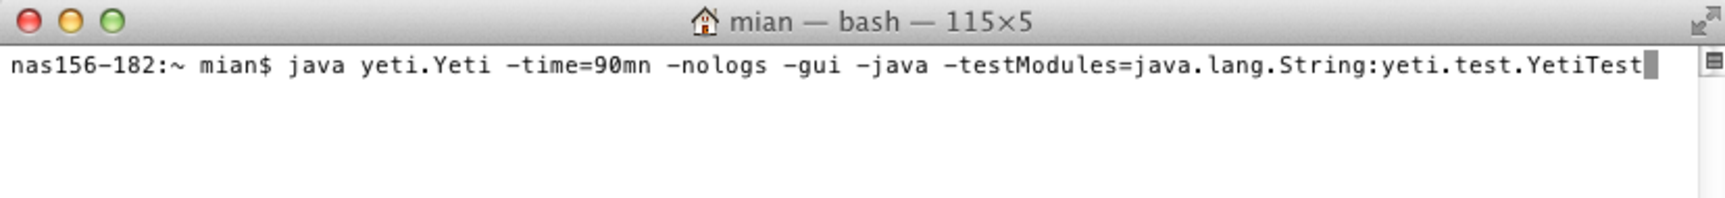
\includegraphics[width= 14cm, height = 1.8cm]{chapter3/yetiCommandCLI.pdf}}
	\caption{Command to launch YETI from CLI}
	\label{fig:yeticommand}
\end{figure}

Alternately, runnable jar file by the name {\it YetiLauncher} is also available to launch YETI from GUI. However, till the writing of this thesis, the GUI version of YETI only supports the basic options of YETI execution. Figure \ref{fig:yetiLauncher} shows the equivalent of above command in GUI mode.

\begin{figure}[h]
	\centering
	\frame{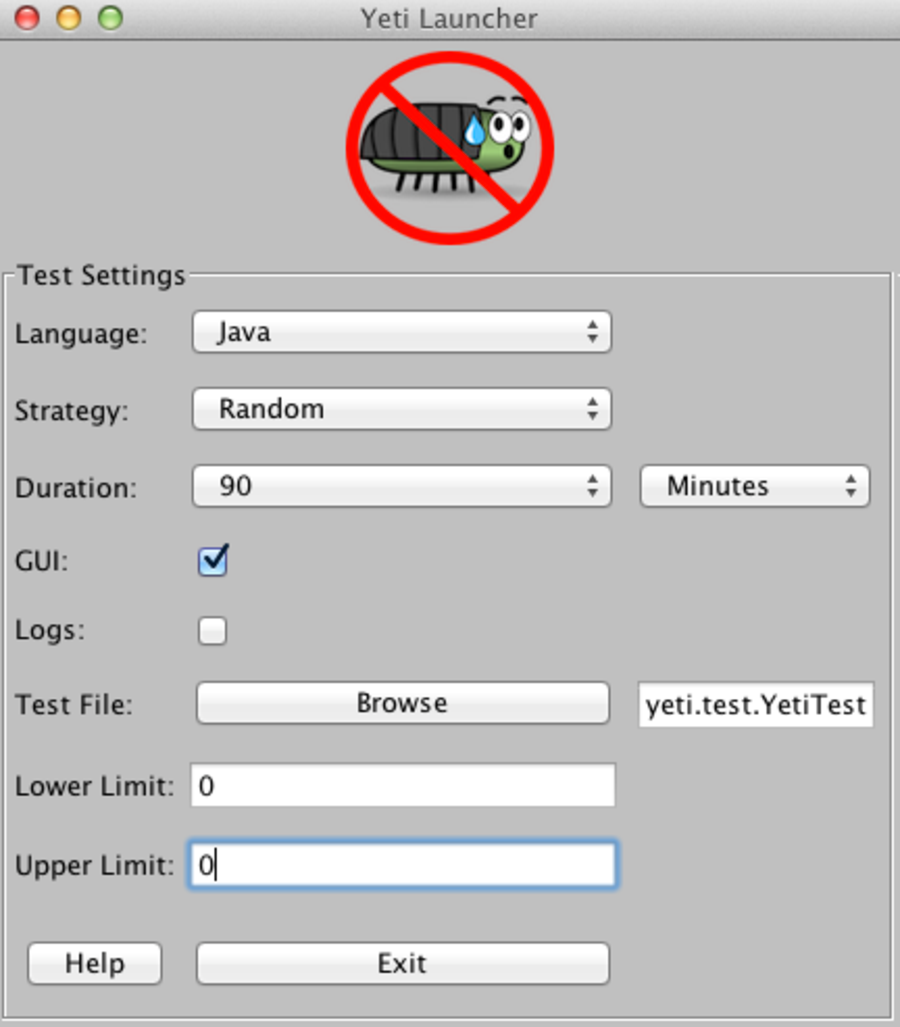
\includegraphics[width= 7cm, height = 8cm]{chapter3/yetiCommandGUI.pdf}}
	\caption{Command to launch YETI from GUI}
	\label{fig:yetiLauncher}
\end{figure}


As a result of both the above commands YETI launch its own GUI window and start testing the assigned programs. 

\subsection{YETI Test Oracle}
Oracles in YETI are language dependant. YETI uses two approaches for oracle (pass/fail judgement). In the presence of program specifications, YETI checks for inconsistencies between the code and the specifications. In the absence of specifications YETI checks for assertion violations if assert statements are included by the programmer. However in the absence of both specifications and assertions YETI performs robustness testing that considers any undeclared runtime exceptions as failures. 

%If code contracts are available, YETI uses them as oracle, however, in their absence YETI uses undeclared runtime exceptions of the underlying language as oracle. The test cases revealing errors are reproduced at the end of each test session for unit and regression testing.
%YETI deals with the oracle problem in two ways. If available, it uses code-contracts as oracles, however in the absence of contracts it uses runtime exceptions as errors which is also known as robustness testing.

\subsection{YETI Report}
YETI gives a complete test report after execution of each test. The report contain all the successful calls with the name of the routines and the unique identifiers for the parameters in each execution. These identifiers are recorded with the assign value to help in debugging the identified fault. 
\begin{figure}[h]
	\centering
	\frame{\includegraphics[width= 7cm, height = 8cm]{chapter3/seecaption.pdf}}
	\caption{YETI successful method calls}
\end{figure}

YETI separates the bugs from successful executions to simplify the test report. This approach helps debuggers to easily track the origin of the problem and rectify it. When a bug is identified during testing YETI saves that state and present it in the bug report. The information includes all the identifiers of the parameters the method call had at the time of execution. It also report the time at which the exception occurs.

\begin{figure}[h]
	\centering
	\frame{\includegraphics[width= 7cm, height = 8cm]{chapter3/seecaption.pdf}}
	\caption{YETI bug reports.}
\end{figure}

subsection{YETI Graphical User Interface}
YETI supports a GUI that not only allows test engineers to monitor the current test session but also to modify its characteristics in real time during test execution. It is useful to have the facility of modifying or aborting the test parameters at run time and observing the test behaviour in response. The figure \ref{fig:yetiGUI} present the YETI GUI comprising of six numbered windows (the windows are labelled for illustration purposes only).

\begin{figure}[h]
	\centering
	\frame{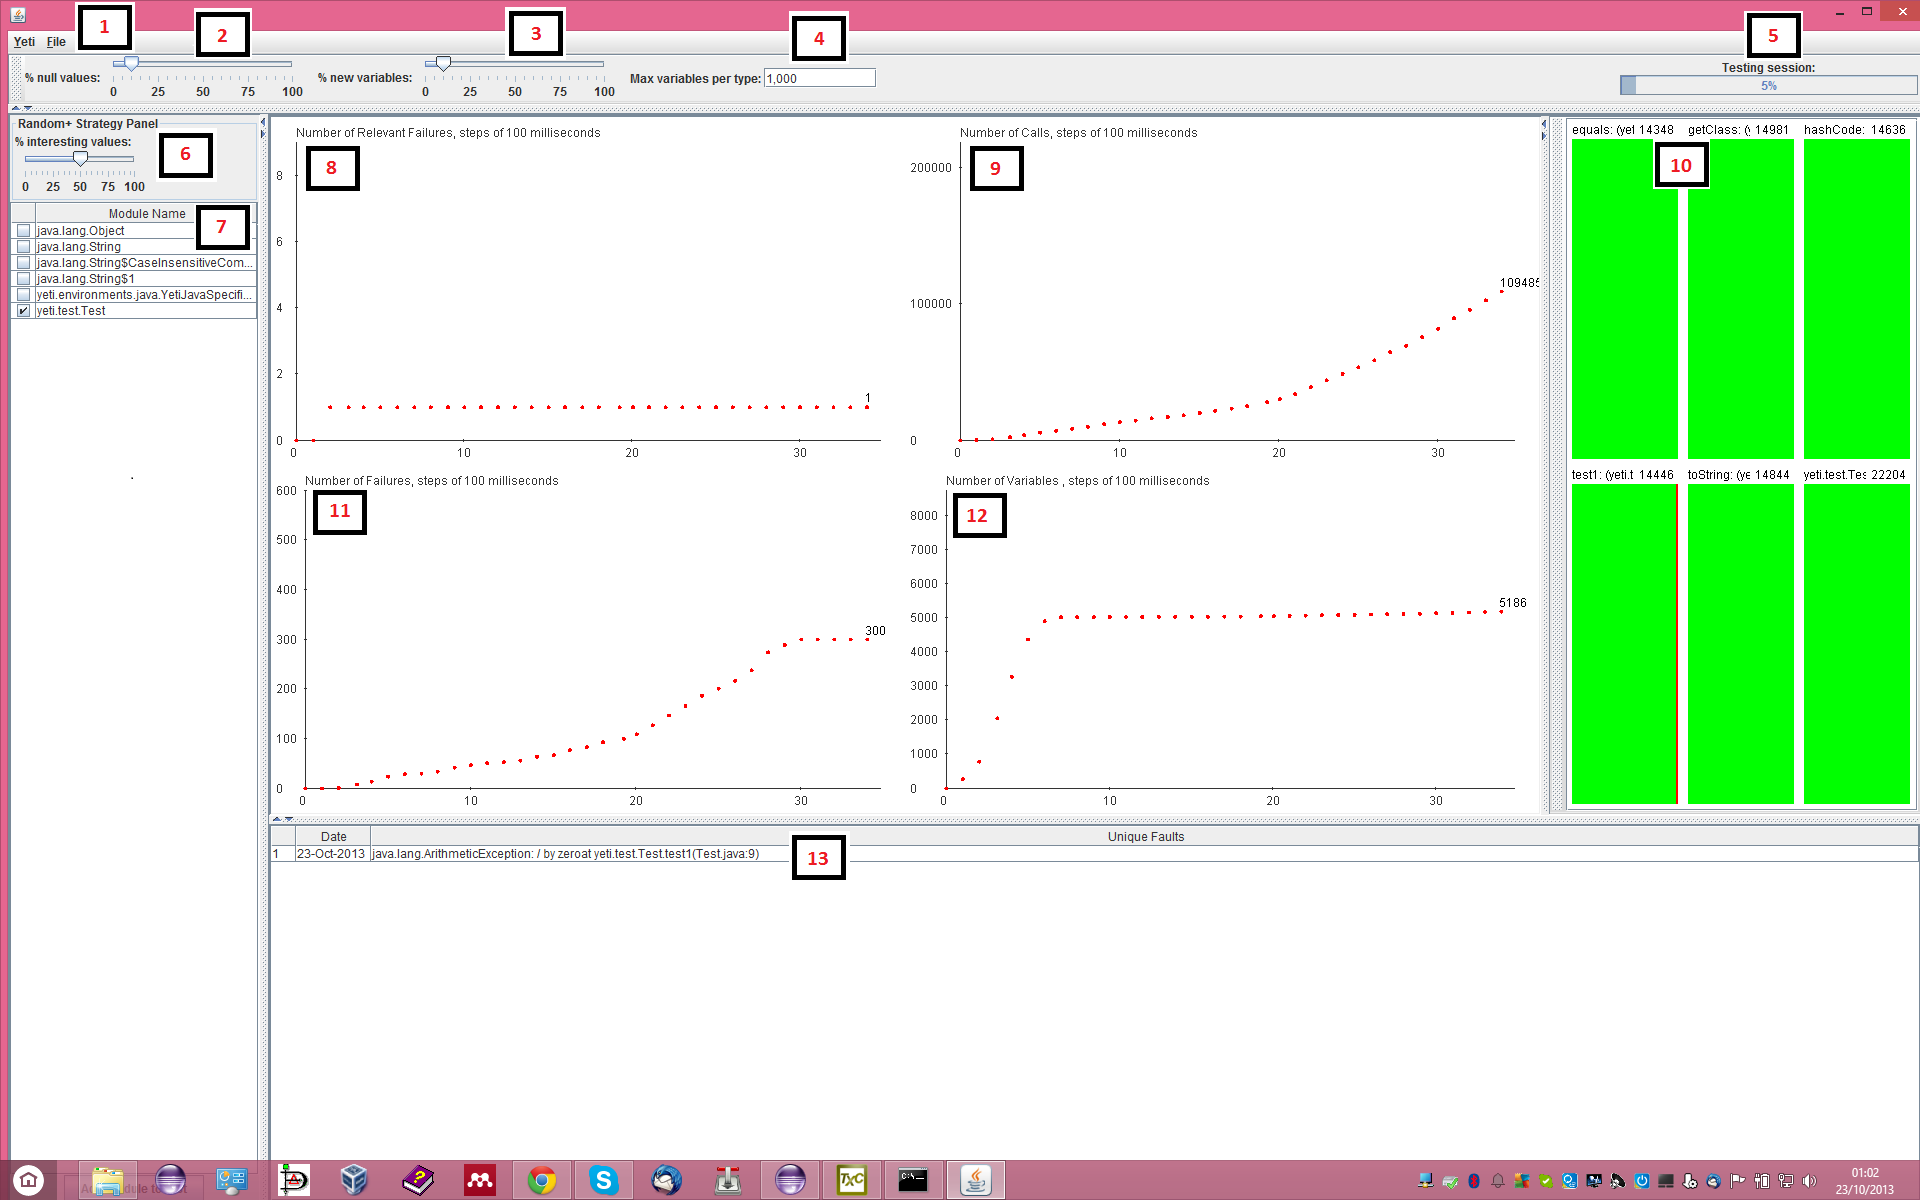
\includegraphics[width= 15cm, height = 12cm]{chapter3/yetiGUI.png}}
	\label{fig:yetiGUI}
	\caption{GUI of YETI Tool}
\end{figure}

\begin{enumerate}
\item Window No 1 displays the failures of the tested module over time.
\item Window No 2 displays the total number of failures over time. These may be generated from calls not related to the tested module.
\item Window No 3 displays the total number of calls to the tested module over time. 
\item Window No 4 displays the total number of variables generated by YETI over time.
\item Window No 5 displays colored rectangles: one for each constructor and method under test. Each rectangle represents the calls to a constructor or a method.
\end{enumerate}
\begin{enumerate}
The colors in a rectangle have the following meaning:
\item Green indicates successful calls (✓). A successful call is one that does not raise an exception or if it does, the method or the constructor declares to throw it.
\item Red indicates failed calls (X). A failed call results from raised RuntimeException or one of its subclasses.
\item Yellow indicates “undecidable” calls (?). A call is “undecidable” if for some reason it takes too long to complete and needs to be stopped, or if a YetiSecurityException (custom exception in YETI) is thrown.
\end{enumerate}


\subsection{Summary of automated testing tools}

\begin{sidewaystable}
    \centering
    \caption{Summary of automated testing tools}
   \begin{tabular}{|l|l|l|l|l|l|l|}
\hline

Tool 				& Language																								& Input  																																			& Strategy 																																											 				& Output		  																								& Benefits																															& Limitations		\\ \hline
JCrasher	  & Java, JML																								& Program																																			& \vtop{\hbox{\strut Method type to predict input,}\hbox{\strut Randomly find values of crash}}  				& TC																													& \vtop{\hbox{\strut Automated TC, Use} \hbox{of Heuristic Rules}} 			& \\ \hline
Jartege			& Java																										& Classes																																			& \vtop{\hbox{\strut Random strategy with controls}\hbox{\strut like weight etc.}} 							 				& TC, RT 																											& Quick, automated																											& \\ \hline
Eclat				& Java																										& Classes, pass TC 																														& \vtop{\hbox{\strut Create model from TC, execute}\hbox{\strut each candidate on the model}} 					& Faulty TC 																									& \vtop{\hbox{\strut produce output text,} \hbox{JML}}									& \\ \hline
Quickcheck	& Haskell																									&	\vtop{\hbox{\strut Specifications}  \hbox{\strut and Functions}}	  			  & \vtop{\hbox{\strut Specification} \hbox{\strut hold to random TC?}} 											 						& Pass/Fail																										& \vtop{\hbox{\strut Easy to use, program} \hbox{documentation}}				&	\\ \hline
Randoop 		& Java, .NET																							& \vtop{\hbox{\strut Specifications,} \hbox{\strut code and time}}					  & \vtop{\hbox{\strut Generate and execute methods} \hbox{\strut \& give feedback for next generation}} 	& Fault TC, RT 																								& 																																			&	\\ \hline
AgitarOne		& Java																										& \vtop{\hbox{\strut Package, time}   \hbox{\strut and manual TC}}						& \vtop{\hbox{\strut Analyse SUT with auto and} \hbox{\strut provided data in specified time}} 					& TC, RT																											& \vtop{\hbox{\strut Eclipse plug-in} \hbox{\& easy to use}}  					& \\ \hline
AutoTest		& Java																										& \vtop{\hbox{\strut Classes, time}   \hbox{\strut and manual TC}} 						& \vtop{\hbox{\strut Heuristic rules} \hbox{\strut to evaluate contracts}} 															& violations, RT 																							& \vtop{\hbox{\strut GUI in HTML,} \hbox{easy to use}} 									& \\ \hline
TestEra			& Java																										& \vtop{\hbox{\strut Specifications,} \hbox{\strut integer \& manual TC}}			& \vtop{\hbox{\strut Check contracts} \hbox{\strut with specifications}} 																& Contracts violations 																				& \vtop{\hbox{\strut short report with} \hbox{faulty TC only}} 					& \\ \hline
Korat 			& Java																										& \vtop{\hbox{\strut Specifications}  \hbox{\strut and manual tests}}					& \vtop{\hbox{\strut Check contracts} \hbox{\strut with specifications}}																& Contracts violations 																				& \vtop{\hbox{\strut GUI, short report} \hbox{with faulty TC only}} 		& \\ \hline
YETI 				& \vtop{\hbox{\strut Java, .NET,}  \hbox{\strut JML}} 		& Code, Time 																																  & RandomPlus, Random 																																										& \vtop{\hbox{\strut Traces of found } \hbox{\strut faults}}	& \vtop{\hbox{\strut GUI, give faulty} \hbox{examples, Quick}} 				& \\ \hline %inserts single line
\end{tabular}
\label{table:Tools}
\end{sidewaystable}


%\begin{figure}[h]
%	\centering
%	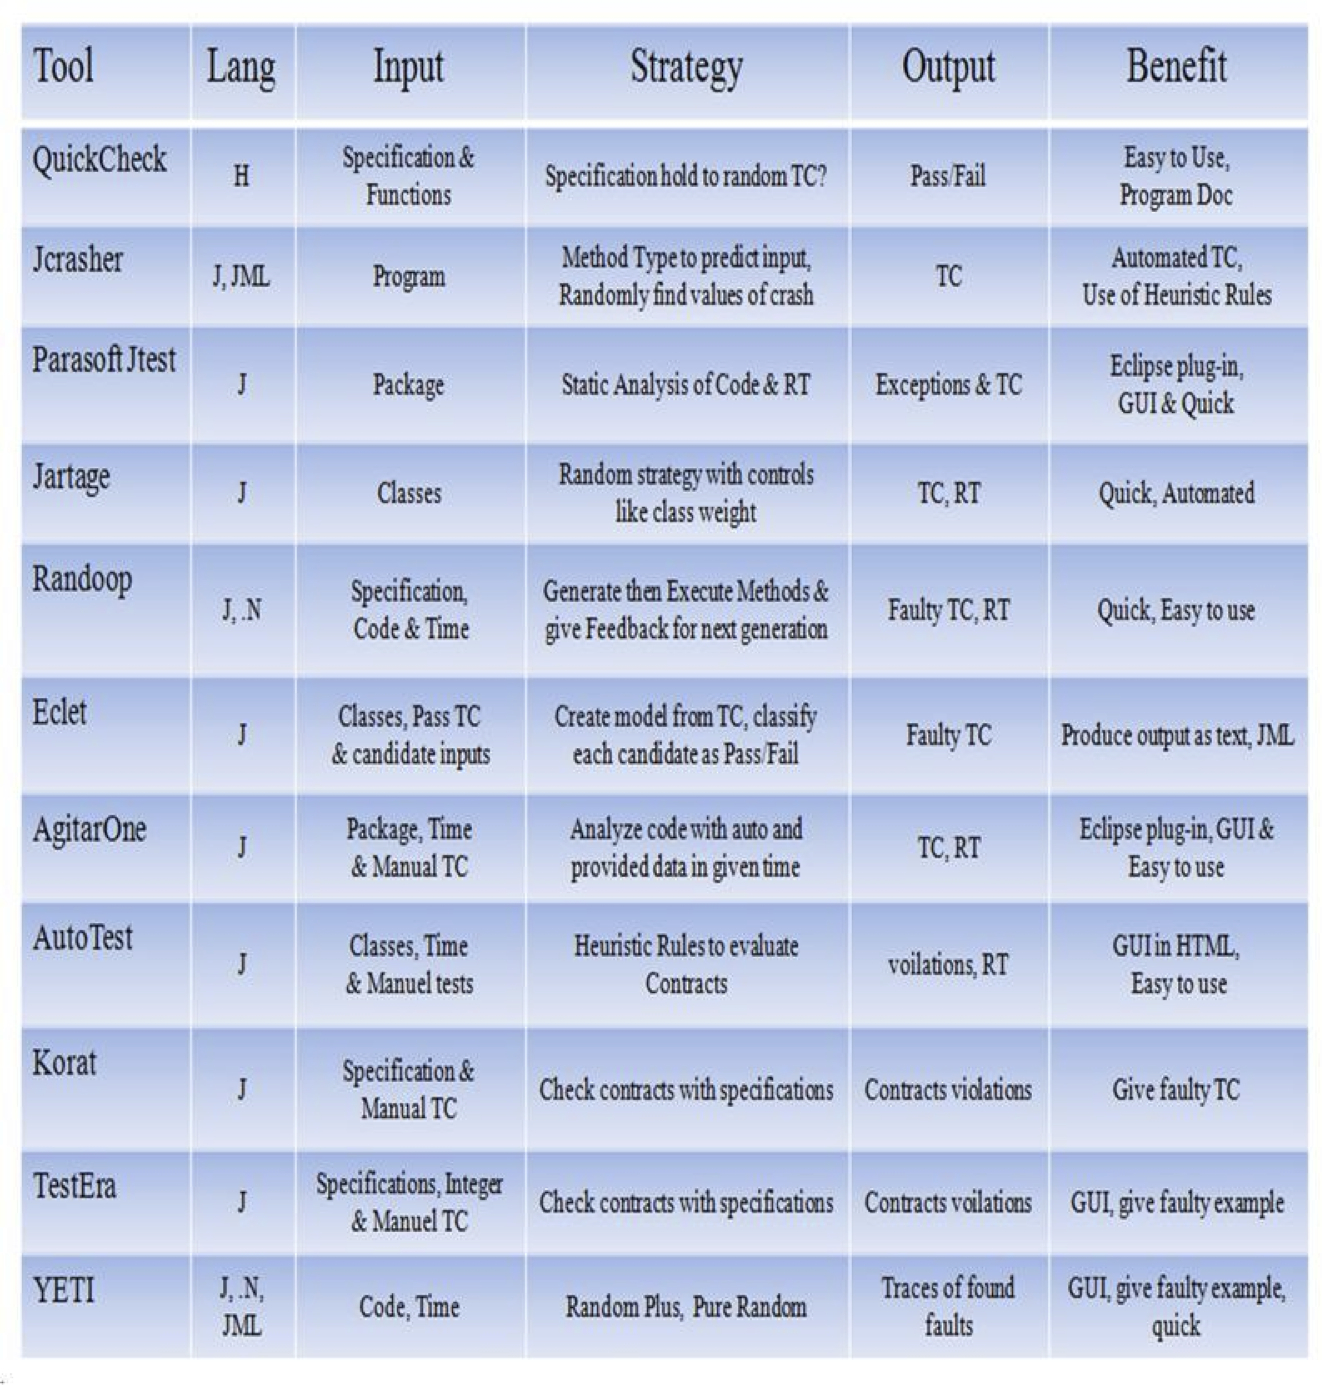
\includegraphics[scale=0.6]{chapter2/tools.jpg}
%	\caption{Summary of automated testing tools}
%\end{figure}


\section{Conclusion}


% ------------------------------------------------------------------------


%%% Local Variables:
%%% mode: latex
%%% TeX-master: "../thesis"
%%% End:
